% Dit is de "preamble" van het document. Hier worden de opmaakopties ingesteld.
% Pro-tip: dingen na het % teken worden niet gecompileerd door LaTeX. Ik zal ze uitgebreid gebruiken om dingen uit te leggen.
% Opmerking: niet om je af te schrikken van LaTeX, maar het is normaal om problemen te hebben. Ik heb de copyright info onderaan het document toegevoegd van de persoon die dit pakket heeft geschreven, omdat zijn documentatie niet helemaal overeenkomt met hoe het daadwerkelijk wordt gebruikt. Dus dit is een combinatie van zijn werkende inleiding samen met mijn toegevoegde commentaar of uitleg. 
% ================================================================

\documentclass[stu,12pt,floatsintext]{apa7}
% Document class input explanation ________________
% LaTeX-bestanden moeten beginnen met de documentklasse, zodat het weet wat het gebruikt.
% - Dit bestand gebruikt de apa7 document class, omdat daar veel opmaak in is ingebouwd.
% Er zijn twee sets haakjes in LaTeX, voor elk commando (de dingen die beginnen met de schuine streep )
% - De tilde haakjes {} zijn verplicht voor het uitvoeren van de opdracht
% - De vierkante haakjes [] zijn opties voor dat commando. Er kan meer dan één set vierkante haakjes zijn voor sommige commando's
% Opties gebruikt in dit document (algemene opmerking - voor elk van deze, als je de andere opties wilt gebruiken, verwissel het dan op die plek in de vierkante haken):
% - stu: this sets the `document mode' as the "student paper" version. Other options are jou (journal), man (manuscript, for journal submission), and doc (a plain document)
% --- De instelling 'student' bevat parameters als 'duedate', 'course' en 'professor' op de titelpagina. Als deze niet gewenst/nodig zijn, gebruik dan de 'man' instelling. De tabellen en figuren worden ook standaard aan het einde van het document toegevoegd. Dit kun je veranderen door de optie 'floatsintext' op te nemen, zoals ik voor jou heb gedaan. Als de docent ze aan het einde wil hebben, verwijder dat dan uit de vierkante haken.
% --- De instelling voor manuscripten is ongeveer wat je zou gebruiken om in te dienen bij een tijdschrift, dus gebruikt 'date' in plaats van 'duedate' en bevat geen informatie over 'course' of 'professor'. Net als bij 'stu' worden tabellen en figuren standaard aan het einde geplaatst in plaats van in de tekst. Dezelfde optie plaatst deze afbeeldingen in de tekst.
% --- Journal ('jou') geeft iets weer dat lijkt op een gewoon tijdschriftformaat - tekst in dubbele kolommen en figuren op hun plaats. Dit kan leuk zijn, vooral als je dit als schrijfvoorbeeld in applicaties gebruikt.
% --- Document ('doc') geeft de tekst weer in één kolom, met één interlinie en figuren op hun plaats. Een alternatieve optie voor het produceren van een meer getypeset uitziend document als schrijfvoorbeeld.
% - 12pt: stelt de lettergrootte in op 12pt. Andere opties zijn 10pt of 11pt
% - floatsintext: zorgt ervoor dat tabellen en figuren in de tekst verschijnen in plaats van aan het einde.

\usepackage[dutch]{babel} % Taalkeuze
\usepackage{hyperref} % Hyperlinks
\usepackage{csquotes} % Noodzakelijk in combinatie met babel.

\usepackage[style=apa,sortcites=true,sorting=nyt,backend=biber]{biblatex}
% biblatex: laadt het pakket dat de bibliografische informatie afhandelt. Een andere optie is natbib, waarmee meer aanpassingen mogelijk zijn
% - style=apa: stelt het referentieformaat in om apa te gebruiken (zij het de 6e editie)
\DeclareLanguageMapping{dutch}{dutch-apa}
\addbibresource{bibliografie.bib} % De bibliografische informatie voor je referenties vanuit Zotero. Dit bestand moet je niet zelf aanmaken, maar exporteren vanuit Zotero (best door de plugin `Better BibTex`: https://retorque.re/zotero-better-bibtex/) en hier uploaden.

\usepackage[T1]{fontenc} 
\usepackage{mathptmx} % Dit is het Times New Roman-lettertype, dat in mijn tijd de norm was. Als je een ander lettertype wilt gebruiken, zie je hier de opties: https://www.overleaf.com/learn/latex/Font_typefaces
% Als alternatief kun je deze twee commando's uitcommentariëren of verwijderen en gewoon het standaardlettertype van Overleaf gebruiken. Zo veel keuzes!

% ================================================================

% Titelpagina _____________________
\title{APA7 \LaTeX{} template met Zotero referentiebeheer voor Wetenschappelijke Methodiek}  % De grote, lange versie van de titel voor de titelpagina.
\shorttitle{\LaTeX{} voor Wetenschappelijke Methodiek}  % De korte titel voor de koptekst.
\author{[Jouw Naam Hier]}
\duedate{\today}
% \date{January 17, 2024}  % De studentenversie gebruikt het commando \datum niet, om wat voor reden dan ook.
\authorsaffiliations{ASO Spijker}
\course{5 Wetenschappelijke Methodiek}  % LaTeX raakt geïrriteerd als dit leeg is, dus zet ik hier iets neer. Als je docent je echter een onvoldoende geeft omdat dit op de titelpagina staat, kun je deze regel leeg laten (verwijder de inhoud, maar laat '\course' staan) en vrede hebben met de fout die dan optreedt. Het document wordt er niet slechter van.
\professor{Pieter Smets}  % Dezelfde situatie als bij de cursusinformatie. Sommige instructeurs willen dit, andere absoluut niet en halen er punten vanaf. Dus doe wat je moet doen.

\abstract{Dit is de samenvatting voor dit artikel waarin de belangrijkste punten van de inleiding, methode, resultaten en discussie snel worden besproken. Waarschijnlijk in meer dan één zin. Durf ik te gokken, meer dan twee? Er is een pagina-einde voordat de inleiding begint.}

\keywords{APA style, voorbeeld, \LaTeX{}, bibliografie, Zotero} % Als je trefwoorden nodig hebt voor je paper, verwijder dan de % aan het begin van deze regel

\begin{document}
\maketitle  % De standaard in LaTeX voor het aanmaken van de titelpagina.

% \section{Introductie}  % Dit commando is uitgecommentarieerd, omdat mij geleerd is dat het overbodig is om de titel en de inleiding van het paper samen te hebben. Als je docent wil dat er "Introductie" staat, verwijder dan de % aan het begin.

Begin je paper met de inleiding. 
Je moet de actieve stem gebruiken in plaats van de passieve stem (de zombiestem).

Dit sjabloon is opgemaakt volgens de richtlijnen van APA Style: marges van één inch boven, onder, links en rechts; lettertype Times New Roman 12 punts; dubbele interlinie; links uitgelijnd; en alinea's ingesprongen. 
Het paginanummer staat een centimeter van de rechterrand op de eerste regel van elke pagina.

Dit sjabloon is geschreven vanuit de situatie van een labrapport, in plaats van andere soorten werkstukken die je misschien schrijft. 
Dit betekent dat de koppen vooraf zijn gevuld met de normale blokken voor dat type werkstuk (bv. methode, resultaten, enz.). 
Als je een ander soort werkstuk schrijft, kun je de koppen en subkoppen naar behoefte toevoegen, verwijderen of wijzigen. 
Voor de duidelijkheid, koppen zijn de belangrijkste onderdelen van het artikel (bv. Inleiding, Methode, enz.). Subkoppen zijn de onderdelen binnen die brokken (bv. Deelnemers, Materialen, enz. in de Methode). 
Dit is iets gemakkelijker te zien in \LaTeX{} door de manier waarop je ermee communiceert en vertelt wat er gebeurt.

Aangezien de inleiding de eerste plaats is waar referenties in papers verschijnen, laten we er nu een paar opnemen. 
Er zijn enkele details waar je op moet letten bij het gebruik van LaTeX {} om je werkstuk te schrijven (ja, er is een LaTeX{} commando om het er zo mooi uit te laten zien, want natuurlijk is dat er). 
Verwijzen naar iets \textbf{in tekst} doe je door de naam in tekst te zetten met het jaartal tussen haakjes; gelukkig voor ons verwerkt \LaTeX{} dit met het juiste commando, zoals \textcite{Sample2024}. 
Wil je misschien gewoon alles opnemen als een tekstbf{parenthetisch}? 
Dat kan ook met \LaTeX{}. 
Bij werken met meerdere auteurs wordt de eerste keer de volledige auteurslijst opgenomen. 
Echter, als die referentie later weer verschijnt, wordt hij ingekort zoals APA het bedoeld had: \parencite{Multiauthor2020}.
Om wat voor reden dan ook lijkt het er niet op dat het multi-auteur werk \parencite[e.g.,][]{Multiauthor2020} werkt zoals het hoort, waar het de volledige lijst geeft de eerste keer dat het wordt opgenomen in de tekst, en daarna wordt ingekort \parencite{Multiauthor2020}. 
Ik weet niet zeker wat er aan de hand is, dus het beste advies dat ik je kan geven is om de eerste instantie zelf uit te schrijven en de rest aan LaTeX over te laten. 
Het is waardeloos, ik weet het. Dat is soms de aard van het beestje LaTeX.

Voor de opmaak moet de pagina Referenties op een nieuwe pagina beginnen. Dit \textit{zou} automatisch geregeld moeten worden door \LaTeX{}, maar het is toch handig om de opmaak te kennen.

Terwijl ik je aandacht heb voordat ik in de secties duik, is er iets dat misschien onopgemerkt voorbijgaat: de \LaTeX{} eigenaardigheid over aanhalingstekens. 
Als je een citaat opneemt met de gewone aanhalingstekens, "ziet het er zo uit". 
De specifieke manier van \LaTeX{} om dit te doen, die net dat beetje extra flair geeft, is om een dubbel vinkje te gebruiken (op de tilde-toets boven op de nummerrij) om het citaat te beginnen, en een dubbele apostrof om het te sluiten. Dan ziet het citaat er ``zo uit''. 
Het zijn ``leuke kleine mannetjes'' die je citaat omhelzen, in plaats van de "meer saaie tekens" die je krijgt van de gewone aanhalingstekens.

Om dit gedeelte af te sluiten, zal ik het tot slot hebben over de inhoud van de inleiding. Denk bij dit soort werkstukken aan het informatieproces in de vorm van een zandloper (blijf bij me, het wordt duidelijk). Het algemene idee is dat je begint op het breedste punt en dan steeds specifieker wordt, totdat je bij het punt van dit artikel bent - de theorie die getest wordt en de hypothese. 
Dan blijf je op dat specifieke detailniveau tot aan de Methoden en Resultaten. 
De Discussie begint specifiek (d.w.z. wat je wel of niet hebt gevonden) en werkt dan terug naar de bredere betekenis of implicaties.

\section{Method}

\subsection{DELETE THIS SECTION - this is an informative section, not something to be included in your final paper.}

I have tried to include the most I've seen asked of students in these papers. You may not need to fill out all of these boxes, in which case you can just delete them. Along with this subsection.

Also, I have seen many different combinations of these boxes - e.g., in one of my papers, I had a ``participants and materials'' section followed by a ``procedure and measures,'' but cannot remember why it was written that way. Maybe it is what the journal wanted? Moral of the story here: go with what the person who is making the decision about the quality of your paper wants. If they want everything in its own little box, do it. If they want some boxes combined, do that.

Just make sure you delete or comment out this subsection!

\subsection{Participants}

Talk about the people who participated in your study. How many students, sourced from where, reimbursed how, ethics assured by what?

\subsection{Materials}

What materials were used in the course of this experiment? Try to walk the line between being overly specific (i.e., ``pens were standard Bic Clio Stic of medium thickness'') while still having enough detail someone else could read your paper and replicate what you used.

Sometimes it can be helpful to include the stimuli used in the experiment. For example, here is an example table (Table \ref{tab:table_words}) of words that were used in this hypothetical experiment. If you make use of the label command, \LaTeX{} will handle numbering things for you.

% There's lots of little components to the table. For the most part you can just copy it, or build your own with Overleaf's table wizard up top. 
% I'll mention that the & character separates items into different columns on a row, and the \\ ends that line. \hline generates a line that matches the width of the table.
\begin{table}
    \caption{Sample words from this hypothetical experiment.}
    \centering
    \begin{tabular}{cc} %The c's here indicate the columns will be centered
        \hline 
         First word & Second word \\
         \hline
         Yeet & Yoink \\
         Hot & Lit \\
         \hline
    \end{tabular}
    \label{tab:table_words}
\end{table}




\subsection{Measures}

This sets up what measure(s) you took during your experiment, including information about \textit{how} those measures were gathered. Was it with some form of worksheet? Was it collected electronically? If electronic, was it through a website or something like E-Prime? If a keyboard was used, were there any specifics about the keys used?

\subsection{Design}

This is typically used to describe the conditions of the experiment. Did everyone experience the same things throughout the experiment, or were there counterbalances, such as for item order exposure, condition order exposure, conditions on days, etc.? 

For undergrad research projects, lab instructors generally try to encourage students towards easier projects, as analyzing a 3 x 2 x 5 experiment is rough, no matter how far along the academic process you are. So I would expect to see something more along the lines of a 2 (experimental manipulation) x 2 (order counterbalance) design.


\subsection{Procedure}

From the time the participant starts the experiment to the time they leave, what did they experience? After informed consent was obtained, what did they do? Or, in some cases, what did you do to them? \textit{What did you do to them?} Make sure you highlight parts where things may deviate from the norm, such as in the debrief, needing to reveal to participants they hadn't been informed of the full nature of the experiment earlier as it would have impacted their ability to respond honestly or otherwise contaminated the data.



\section{Results}

Some instructors will want things broken down with the subheadings (e.g., `Descriptive Statistics') I have included, some will light your paper on fire if you \textit{do} include these. Always check with the assignment/rubric for what is wanted. Also, don't check my math on these, I am making all of the numbers up as we go, so it's almost certainly not going to hang together correctly.

I'll add this tip in here: since \LaTeX{} uses the percent symbol as the signal to comment out/hide what's typed after it in that line, what do you do if you need that symbol? You add what's called the `escape character' in front of it - the backslash. So, it would look like this: 21\%. Boom, you've got a percent symbol in text. Same goes for an ampersand: \&.

\subsection{Descriptive Statistics}

In this portion, you describe the data obtained. This includes things like the counts, means, and standard deviations. This may be omitted or rolled into the rest of the statistical discussion, so as always, check with what is being asked of you. If it is wanted as a separate section, check to see if it would be acceptable to include things as a table, a figure, or if it would be better to write it out in text. We are going to use a figure.

\begin{figure}
    \centering
    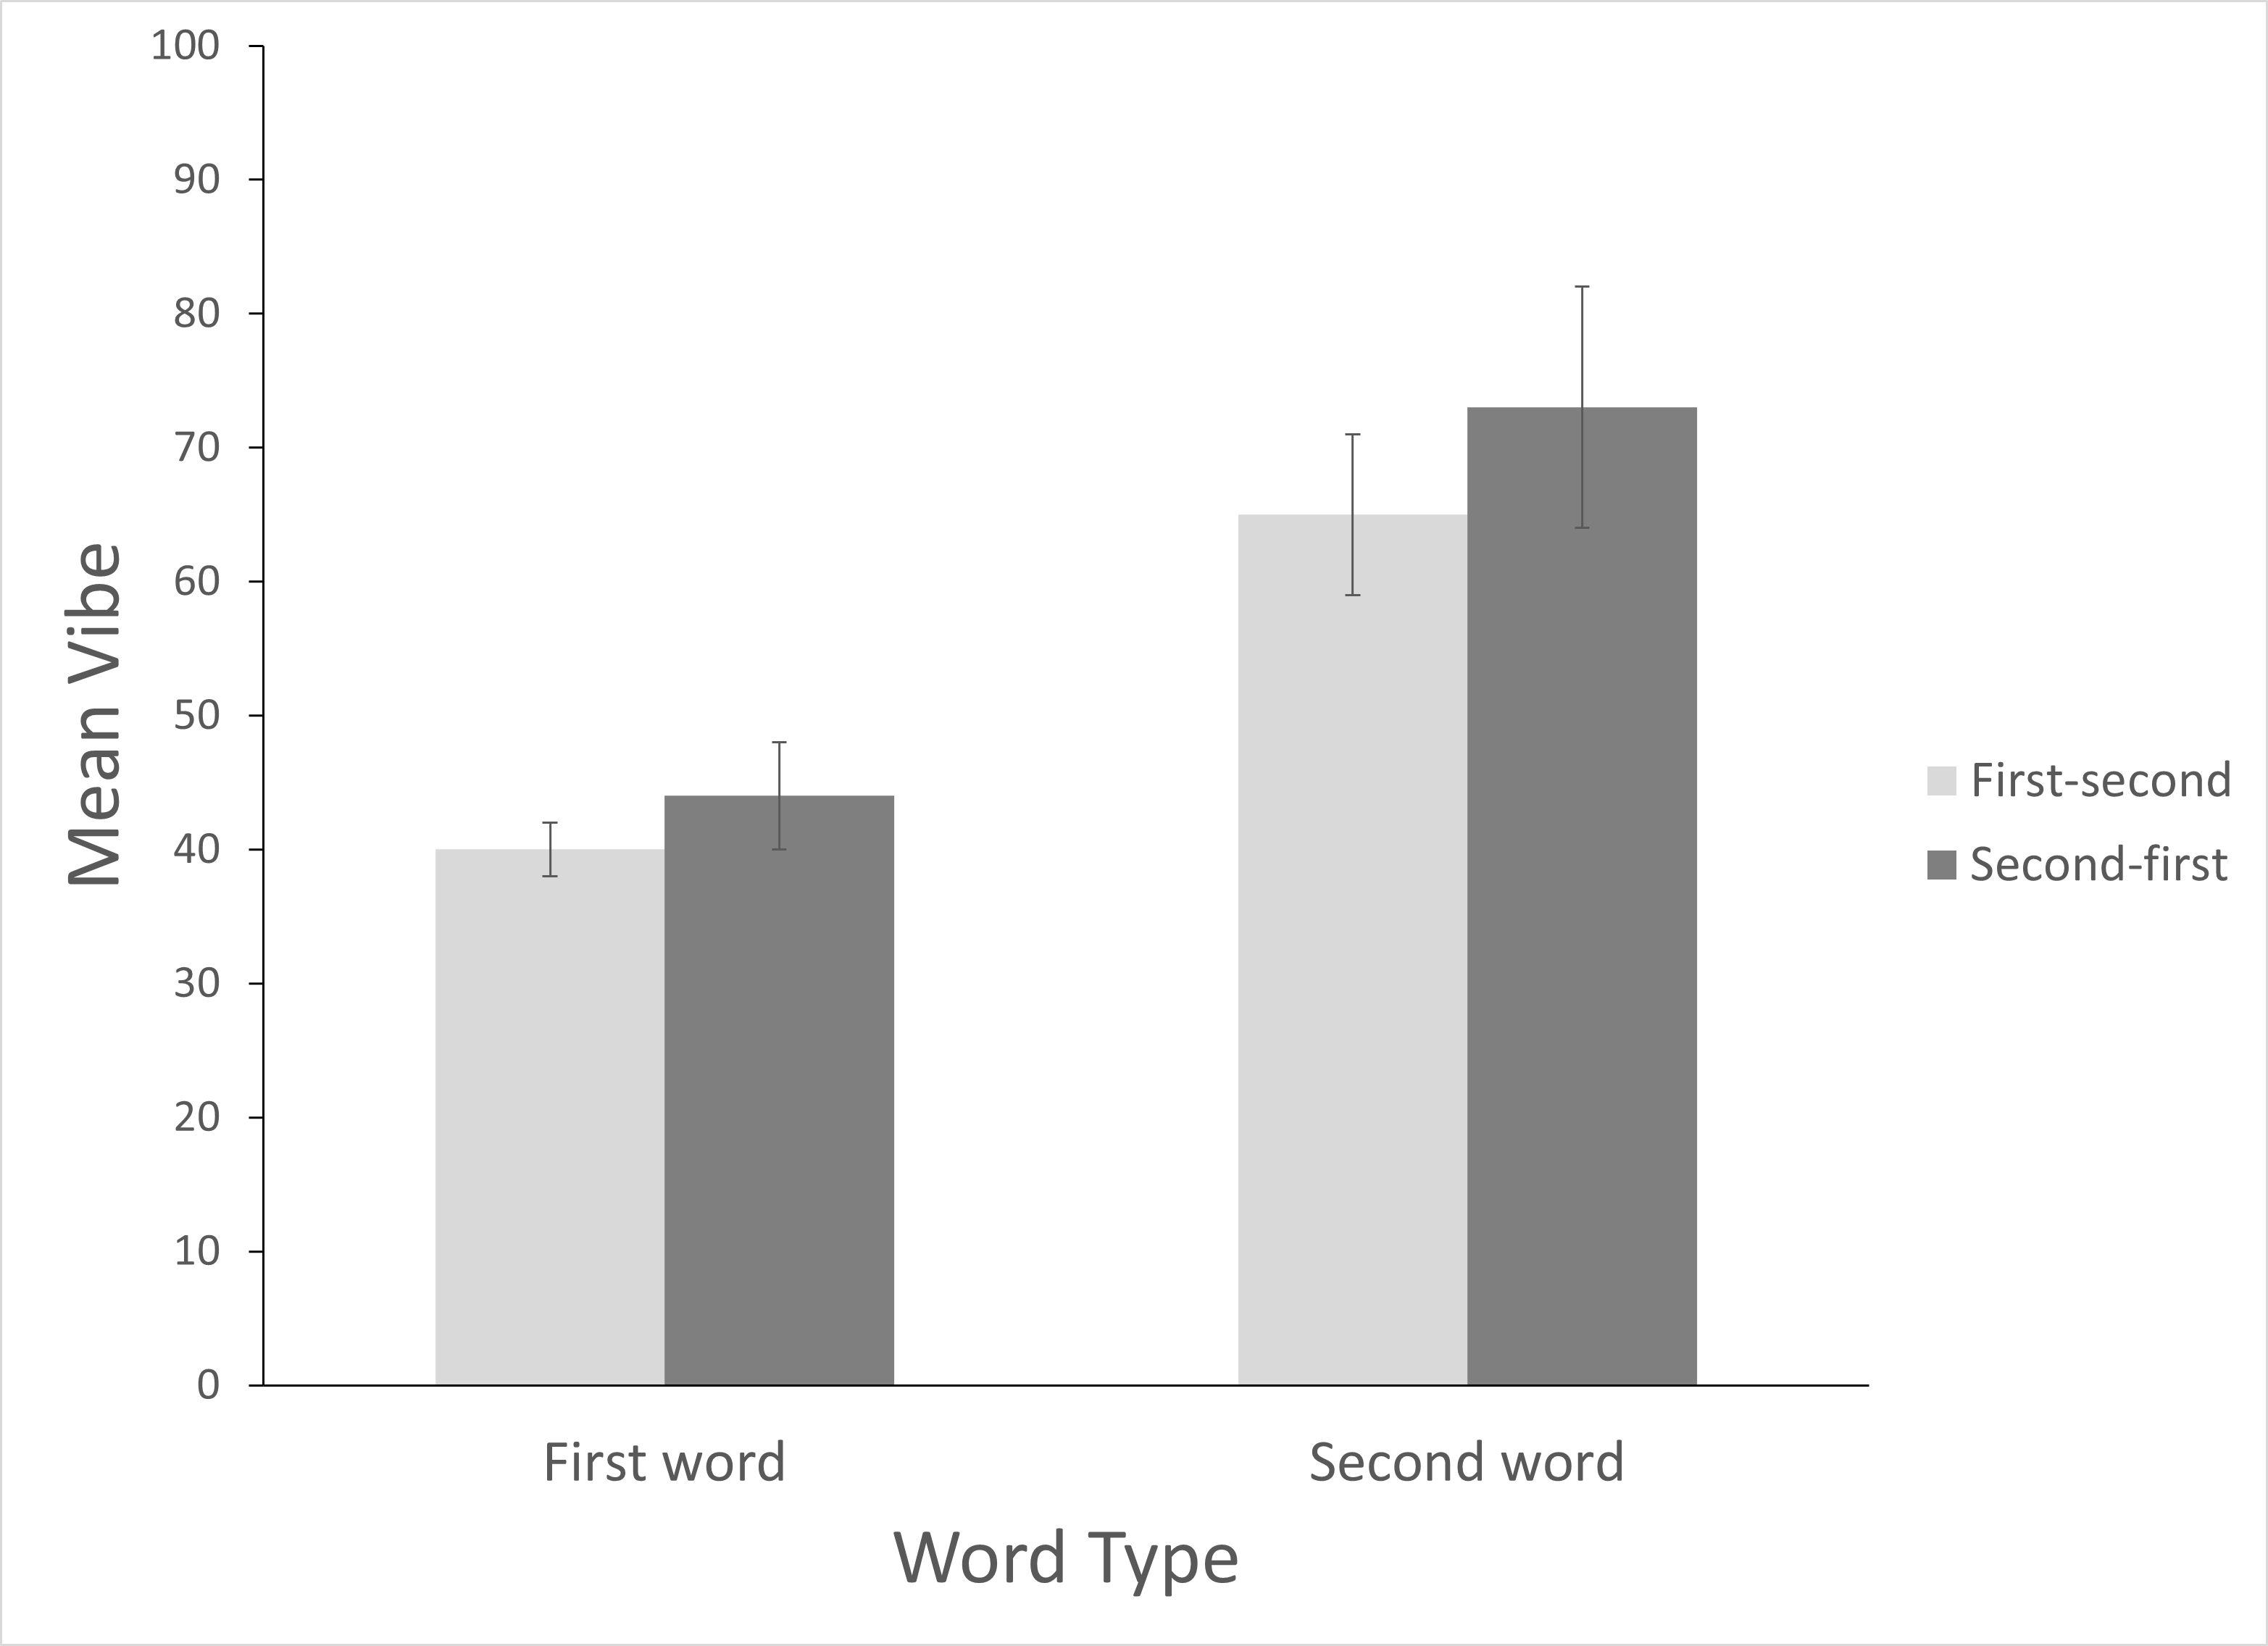
\includegraphics[width=0.75\linewidth]{sampleFig.png} % This is setting the figure to be .75x the width of the line. This can go all the way from 0.1 to 1 (and beyond, but then you're outside the page).
    \caption{The mean vibes for each word type and counterbalanced condition order. Error bars represent one standard error of the mean.}
    \label{fig:OverallEffect}
\end{figure}

Figure~\ref{fig:OverallEffect} shows the means and standard errors for the four experimental groups. As shown, the mean vibes for the second word ($M = $ 69, $SE = $ 7.5) were greater than the first word ($M = $ 42, $SE = $ 3), but roughly equivalent between presentation order conditions. Another fun little \LaTeX{} thing here: your instructor may explicitly want you to use $M$, but one of \LaTeX{}'s strengths is the easy of ``math mode'' (i.e., everything enclosed by the dollar signs). %In math mode, you can easily throw in Greek characters. So you \textit{could} instead present the descriptive statistics as ($\mu = $ 42). Oooh. Shiny. Although that seems to make Overleaf work extra hard, so I keep seeing a message encouraging upgrading to a paid plan, so I've commented this part out.

\subsection{Inferential Statistics}

This is where you start to do the actual statistical analysis. We generally tell students not to \textit{interpret} what the results mean until the discussion, but pay attention when reading journal articles - realistically a bit of interpretation does tend to happen at this point in published works.

A benefit of using \LaTeX{} is the ease in adding in macros to simplify your life. A common place I rolled these out in my dissertation were to make the formatting of all the analyses correct without a lot of work. I will include a couple example macros in the editor-side now, then use them in text. But, \textbf{another pro tip:} if you are going to deploy these macros, I would get in the habit of putting them up in the preamble so they are easier to find. Also, if you really get on board the \LaTeX{} train (which you should), you can recycle the preamble between projects, so those macros will also come along for the ride.

% A macro will have this format \newcommand{macroNameYoullUseToCallIt}[Number of inputs]{What the macro does} 
% The #s indicate where information will be slotted in when the macro is used
% The dollar signs indicate "math mode" is being used. It's mandatory for some functionality (like super/subscripts) or accessing the Greek alphabet used in statistical reporting.
% These macros are including the amount of info we expected from students when I was TAing labs. You can fill them out further if more info is required - just make sure you update the number in the square brackets!
\newcommand{\ttestSig}[2]{$t$(#1) = #2, $p < .05$}
\newcommand{\ttestInsig}[2]{$t$(#1) = #2, $p > .05$}
\newcommand{\anovaSig}[3]{$F$(#1,#2) = #3, $p < .05$}
\newcommand{\anovaInsig}[3]{$F$(#1,#2) = #3, $p > .05$}

Using the hypothetical experiment we have set up, let's say there was a significant interaction found between the word conditions (first versus second) and exposure order (first-second versus second-first), \anovaSig{11}{111}{4.20}. Pairwise comparisons indicate that this was driven by the words themselves, as there was a significant difference between the words, \ttestSig{111}{3.21}, but not for the exposure order, \ttestInsig{111}{.42}.

\section{Discussion}

Zoals vermeld aan het einde van de Introductie, begint de Discussie specifiek voordat het een breder beeld schetst. Dit betekent meestal dat de discussie begint met een herhaling van de resultaten, met meer nadruk op de interpretatie. Welke verschillen zijn er wel (of niet) gevonden? Ondersteunt dit je voorspellingen, of heb je de nulhypothese niet verworpen? Verklaringen van die aard.


Als je dat gedaan hebt, kun je je bevindingen koppelen aan de bestaande literatuur. Misschien ondersteunt dit resultaat het werk van \textcite{Contributor2023} maar spreekt het anderen tegen \parencite[bv.,][]{Sample2024}.  % De extra vierkante haakjes hier vertellen LaTeX dat de bv., vooraan moet staan; het lijkt er anders van uit te gaan dat de bv., na het citaat hoort. Merk ook op dat ik deze opmerking hier kan plaatsen zonder de alinea af te breken. Je hebt een dubbele regeleinde nodig om paragrafen te scheiden.
Waarom zou dit het geval kunnen zijn? Welke overeenkomsten of verschillen bestaan er tussen jouw experiment en de andere werken die de verschillen zouden kunnen verklaren? Of als de resultaten vergelijkbaar zijn, wat betekent dit dan voor de kerntheorie (bijvoorbeeld, laat het zien dat het stand houdt met andere stimuli, of in een andere context, of met een andere timing, etc.).

Het is ook belangrijk om te werken met mogelijke beperkingen van je werk. In cognitieve labrapporten voor studenten gaat het vaak over de steekproefgrootte. Het kan moeilijk zijn om significantie te bereiken als je een steekproefgrootte van 10 hebt. Andere veelvoorkomende beperkingen kunnen dingen zijn zoals de stimuli werkten niet zoals je had gehoopt, de deelnemers begrepen de aanwijzingen voor het experiment niet (of waren niet op de hoogte van wat je aan het testen was waardoor hun gegevens vertekend werden), of dingen die je opmerkt tijdens het uitvoeren van het experiment die je anders zou doen als je het in de toekomst opnieuw zou doen.

Sluit af met een korte samenvatting van je bevindingen, wat het betekent voor de theorie die je aan het testen was en wat het zou kunnen betekenen voor toekomstig onderzoek. 
Veel schrijfplezier!


\printbibliography

\end{document}

%% 
%% Copyright (C) 2019 by Daniel A. Weiss <daniel.weiss.led at gmail.com>
%% 
%% This work may be distributed and/or modified under the
%% conditions of the LaTeX Project Public License (LPPL), either
%% version 1.3c of this license or (at your option) any later
%% version.  The latest version of this license is in the file:
%% 
%% http://www.latex-project.org/lppl.txt
%% 
%% Users may freely modify these files without permission, as long as the
%% copyright line and this statement are maintained intact.
%% 
%% This work is not endorsed by, affiliated with, or probably even known
%% by, the American Psychological Association.
%% 
%% This work is "maintained" (as per LPPL maintenance status) by
%% Daniel A. Weiss.
%% 
%% This work consists of the file  apa7.dtx
%% and the derived files           apa7.ins,
%%                                 apa7.cls,
%%                                 apa7.pdf,
%%                                 README,
%%                                 APA7american.txt,
%%                                 APA7british.txt,
%%                                 APA7dutch.txt,
%%                                 APA7english.txt,
%%                                 APA7german.txt,
%%                                 APA7ngerman.txt,
%%                                 APA7greek.txt,
%%                                 APA7czech.txt,
%%                                 APA7turkish.txt,
%%                                 APA7endfloat.cfg,
%%                                 Figure1.pdf,
%%                                 shortsample.tex,
%%                                 longsample.tex, and
%%                                 bibliography.bib.
%% 
%%
%%
%% This is file `./samples/shortsample.tex',
%% generated with the docstrip utility.
%%
%% The original source files were:
%%
%% apa7.dtx  (with options: `shortsample')
%% ----------------------------------------------------------------------
%% 
%% apa7 - A LaTeX class for formatting documents in compliance with the
%% American Psychological Association's Publication Manual, 7th edition
%% 
%% Copyright (C) 2019 by Daniel A. Weiss <daniel.weiss.led at gmail.com>
%% 
%% This work may be distributed and/or modified under the
%% conditions of the LaTeX Project Public License (LPPL), either
%% version 1.3c of this license or (at your option) any later
%% version.  The latest version of this license is in the file:
%% 
%% http://www.latex-project.org/lppl.txt
%% 
%% Users may freely modify these files without permission, as long as the
%% copyright line and this statement are maintained intact.
%% 
%% This work is not endorsed by, affiliated with, or probably even known
%% by, the American Psychological Association.
%% 
%% ----------------------------------------------------------------------